\documentclass[12pt, a4paper, twoside]{article}
\usepackage[utf8]{inputenc}
\usepackage[spanish]{babel}
\usepackage{hyperref}
\usepackage{fancyhdr}
\usepackage{graphicx}
\usepackage{enumitem}

\pagestyle{fancy}
\fancyhf{}
\fancyfoot[R]{\thepage}
\fancyfoot[L]{\nouppercase{\leftmark}}
\fancyhead[R]{Mapas Conceptuales.}
\fancyhead[L]{Carlos G. Pérez Aranda. }

\graphicspath{{./Images/}}
\title{Mapas Conceptuales}
\author{Carlos G. Pérez Aranda}
\date{2025}
\begin{document}
\maketitle

\section{¿Qué son los Mapas Conceptuales?}
Un mapa conceptual es una herramienta gráfica que permite representar y 
organizar información de manera visual. Se utiliza para mostrar 
relaciones entre conceptos, ideas o temas, facilitando la comprensión y 
el aprendizaje. Los mapas conceptuales son especialmente útiles en el 
ámbito educativo, ya que ayudan a los estudiantes a estructurar y 
sintetizar información compleja.

\section{Características de los Mapas Conceptuales}
\begin{itemize}
    \item \textbf{Conceptos:} Los conceptos son las ideas o temas que se representan en el mapa conceptual. Se suelen escribir en forma de palabras o frases cortas.
    \item \textbf{Conectores:} Los conectores son palabras o frases que indican la relación entre los conceptos. Pueden ser verbos, preposiciones o frases que describen la relación.
    \item \textbf{Jerarquía:} Los mapas conceptuales tienen una estructura jerárquica, donde los conceptos más generales se encuentran en la parte superior y los conceptos más específicos en la parte inferior.
    \item \textbf{Estructura:} La estructura del mapa conceptual es flexible y puede adaptarse a diferentes estilos de aprendizaje y necesidades.
    \item \textbf{Visualización:} Los mapas conceptuales utilizan elementos visuales como colores, formas y líneas para facilitar la comprensión y el análisis de la información.
\end{itemize}
\section{Uso de los Mapas Conceptuales}
Los mapas conceptuales son una herramienta versátil que se puede utilizar 
en diversas áreas, como la educación, el trabajo y la vida personal. 
Algunas aplicaciones comunes de los mapas conceptuales incluyen:
\begin{itemize}
    \item \textbf{Toma de notas:} Los mapas conceptuales son una excelente herramienta para tomar notas durante clases, conferencias o reuniones, permitiendo organizar la información de manera clara y estructurada.
    \item \textbf{Planificación de proyectos:} Los mapas conceptuales son útiles para planificar proyectos, estableciendo objetivos, tareas y plazos de manera visual y organizada.
    \item \textbf{Resolución de problemas:} Los mapas conceptuales pueden ayudar a identificar y analizar problemas, facilitando la búsqueda de soluciones creativas y efectivas.
    \item \textbf{Estudio:} Los mapas conceptuales son una herramienta eficaz para estudiar y repasar información, facilitando la memorización y comprensión de conceptos complejos.
    \item \textbf{Brainstorming:} Los mapas conceptuales son ideales para sesiones de brainstorming, permitiendo generar ideas y establecer conexiones entre ellas de manera visual.
    \item \textbf{Presentaciones:} Los mapas conceptuales pueden utilizarse como apoyo visual en presentaciones, facilitando la comprensión y el análisis de la información presentada.
    \item \textbf{Creatividad:} La creación de mapas conceptuales estimula la creatividad y el pensamiento lateral, permitiendo explorar nuevas ideas y enfoques.
    \item \textbf{Organización:} Los mapas conceptuales permiten organizar la información de manera clara y estructurada, facilitando el análisis y la síntesis de ideas.
    \item \textbf{Memorización:} La representación visual de las ideas y conceptos en un mapa conceptual facilita la memorización y el recuerdo de la información.
    \item \textbf{Síntesis:} Los mapas conceptuales permiten sintetizar información compleja, resumiendo las ideas principales y facilitando su comprensión.
    \item \textbf{Análisis:} La estructura jerárquica de los mapas conceptuales facilita el análisis de la información, permitiendo identificar relaciones y conexiones entre conceptos.
    \item \textbf{Organización de ideas:} Los mapas conceptuales son una herramienta eficaz para organizar ideas y conceptos, facilitando la planificación y el desarrollo de proyectos.
\end{itemize}
\section{Ejemplo de Mapa Conceptual}
\begin{figure}[h]
    \centering
    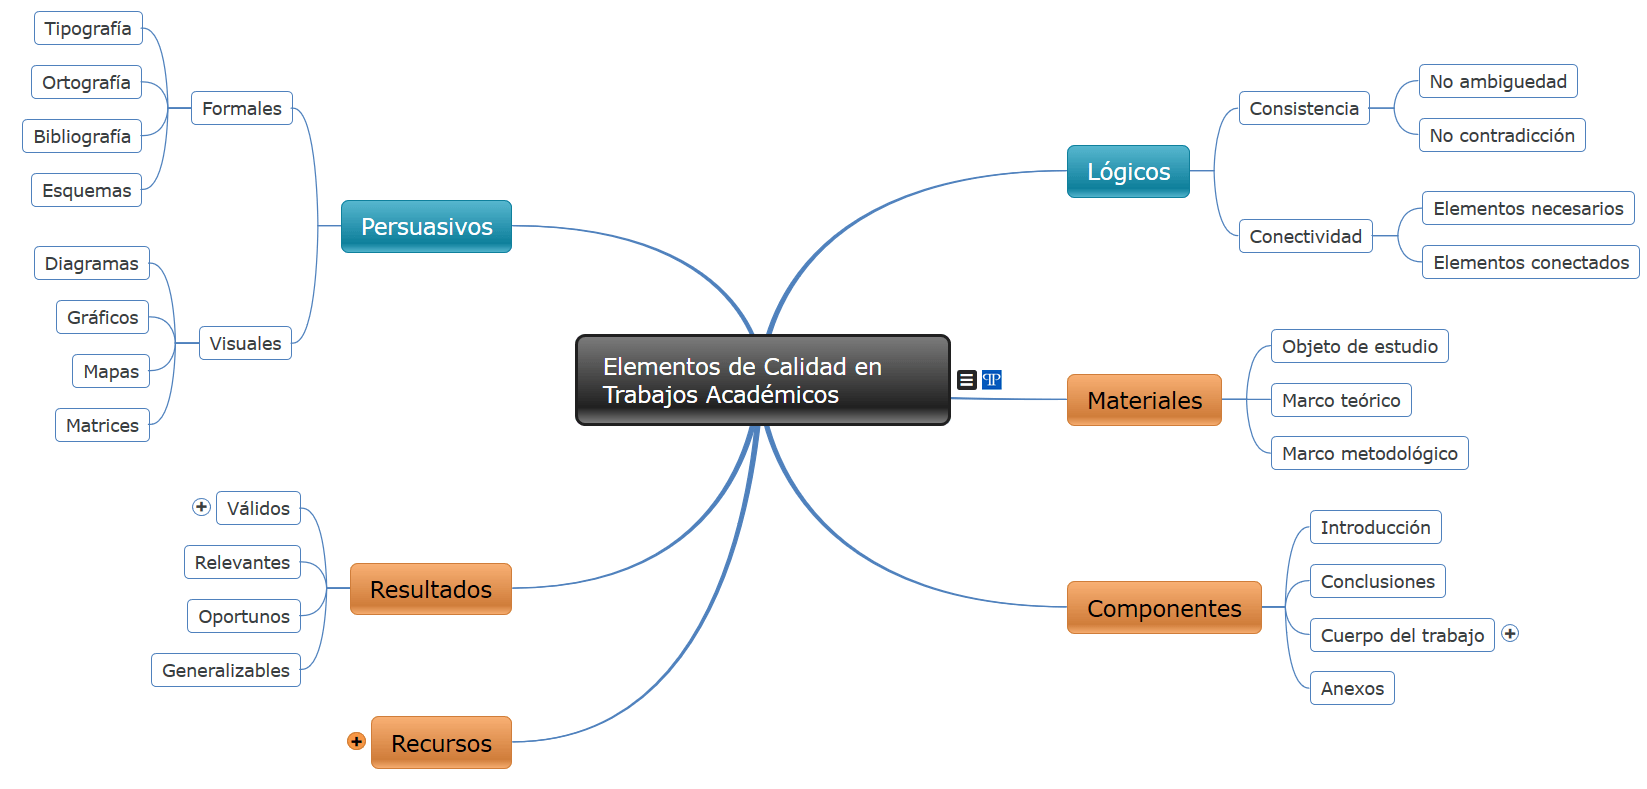
\includegraphics[width=0.8\textwidth]{ejemplomc.png}
    \caption{Ejemplo de Mapa Conceptual}
    \label{fig:mapa_conceptual}
\end{figure}
\section{Descripción del programa CmapTools}
CmapTools es un software diseñado para crear mapas conceptuales de manera sencilla y efectiva. 
Permite a los usuarios construir, editar y compartir mapas conceptuales 
de forma colaborativa. Algunas características destacadas de CmapTools que hacen que sea 
mi herramienta elegida son:
\begin{itemize}
    \item Interfaz intuitiva y fácil de usar.
    \item Herramientas de edición y personalización de mapas conceptuales.
    \item Posibilidad de agregar imágenes, enlaces y notas a los conceptos.
    \item Funciones de colaboración en línea para trabajar en equipo.
    \item Exportación e importación de mapas conceptuales en diferentes formatos.
    \item Integración con otras aplicaciones y plataformas educativas.
    \item Acceso a una amplia biblioteca de recursos y ejemplos de mapas conceptuales.
    \item Soporte para múltiples idiomas.
\end{itemize}

\end{document}